\documentclass[9pt, aspectratio=169]{beamer}

\usetheme{metropolis}
\setbeamertemplate{itemize items}{\faAngleRight}

\metroset{titleformat=smallcaps,block=fill,numbering=counter,progressbar=frametitle,sectionpage=none}
\setbeamersize{text margin left=5mm,text margin right=5mm} 
% %%%%%%%%%%%%%%%%%%%%%%%%%%%%%%%%%%%%%%%%%%%%%%%%%%%%%%%%%%%%%%%%%%%%%%%%%%%%%%
% \embedvideo{<poster or text>}{<video file (MP4+H264)>}
% \embedvideo*{...}{...}                     % auto-play
%%%%%%%%%%%%%%%%%%%%%%%%%%%%%%%%%%%%%%%%%%%%%%%%%%%%%%%%%%%%%%%%%%%%%%%%%%%%%%

\usepackage[bigfiles]{pdfbase}
\ExplSyntaxOn
\NewDocumentCommand\embedvideo{smm}{
  \group_begin:
  \leavevmode
  \tl_if_exist:cTF{file_\file_mdfive_hash:n{#3}}{
    \tl_set_eq:Nc\video{file_\file_mdfive_hash:n{#3}}
  }{
    \IfFileExists{#3}{}{\GenericError{}{File~`#3'~not~found}{}{}}
    \pbs_pdfobj:nnn{}{fstream}{{}{#3}}
    \pbs_pdfobj:nnn{}{dict}{
      /Type/Filespec/F~(#3)/UF~(#3)
      /EF~<</F~\pbs_pdflastobj:>>
    }
    \tl_set:Nx\video{\pbs_pdflastobj:}
    \tl_gset_eq:cN{file_\file_mdfive_hash:n{#3}}\video
  }
  %
  \pbs_pdfobj:nnn{}{dict}{
    /Type/RichMediaInstance/Subtype/Video
    /Asset~\video
    /Params~<</FlashVars (
      source=#3&
      skin=SkinOverAllNoFullNoCaption.swf&
      skinAutoHide=true&
      skinBackgroundColor=0x5F5F5F&
      skinBackgroundAlpha=0
    )>>
  }
  %
  \pbs_pdfobj:nnn{}{dict}{
    /Type/RichMediaConfiguration/Subtype/Video
    /Instances~[\pbs_pdflastobj:]
  }
  %
  \pbs_pdfobj:nnn{}{dict}{
    /Type/RichMediaContent
    /Assets~<<
      /Names~[(#3)~\video]
    >>
    /Configurations~[\pbs_pdflastobj:]
  }
  \tl_set:Nx\rmcontent{\pbs_pdflastobj:}
  %
  \pbs_pdfobj:nnn{}{dict}{
    /Activation~<<
      /Condition/\IfBooleanTF{#1}{PV}{XA}
      /Presentation~<</Style/Embedded>>
    >>
    /Deactivation~<</Condition/PI>>
  }
  %
  \hbox_set:Nn\l_tmpa_box{#2}
  \tl_set:Nx\l_box_wd_tl{\dim_use:N\box_wd:N\l_tmpa_box}
  \tl_set:Nx\l_box_ht_tl{\dim_use:N\box_ht:N\l_tmpa_box}
  \tl_set:Nx\l_box_dp_tl{\dim_use:N\box_dp:N\l_tmpa_box}
  \pbs_pdfxform:nnnnn{1}{1}{}{}{\l_tmpa_box}
  %
  \pbs_pdfannot:nnnn{\l_box_wd_tl}{\l_box_ht_tl}{\l_box_dp_tl}{
    /Subtype/RichMedia
    /BS~<</W~0/S/S>>
    /Contents~(embedded~video~file:#3)
    /NM~(rma:#3)
    /AP~<</N~\pbs_pdflastxform:>>
    /RichMediaSettings~\pbs_pdflastobj:
    /RichMediaContent~\rmcontent
  }
  \phantom{#2}
  \group_end:
}
\ExplSyntaxOff
%%%%%%%%%%%%%%%%%%%%%%%%%%%%%%%%%%%%%%%%%%%%%%%%%%%%%%%%%%%%%%%%%%%%%%%%%%%%%%

\usepackage{fontspec,minted}
\usepackage[scale=1]{ccicons}
\usepackage{metalogo}
\usepackage{xcolor,colortbl}
\usepackage{multicol,multirow,booktabs}
\usepackage{appendixnumberbeamer}
\usepackage{graphicx}
\usepackage{bm}
\usepackage{fontawesome}
\usepackage{csquotes}
\usepackage[backend=biber, natbib, sorting=nyt, doi=true, url=false, url=false, isbn=false, maxbibnames=10]{biblatex}
\addbibresource{../../utils/refs.bib}

\usepackage[spanish]{babel}
\usepackage{mathtools}
\usefonttheme{professionalfonts}
\usepackage{textcomp}

\setsansfont[BoldFont={Iwona Bold}, Numbers={Lining, Proportional}]{Iwona Light}
% \setmathsfont(Digits)[Numbers={Lining, Proportional}]{Fira Sans Light}
\setmonofont[Scale=MatchLowercase]{DejaVu Sans Mono}

\setbeamercolor{alerted text}{fg=red,bg=black!2}
\setbeamercolor{progress bar}{fg=red,bg=red!2}
\setbeamertemplate{itemize item}{\faCaretRight}
\setbeamertemplate{itemize subitem}{ \faAngleRight}
\setbeamertemplate{blocks}[shadow=false]
\setbeamercolor{block title}{bg=black!30,fg=red}
\setbeamercolor{block body}{bg=black!20,fg=black}
 
\usepackage{gensymb,amssymb}
\usepackage{upquote}
\usepackage{algpseudocode}
\algrenewcommand\algorithmicrequire{\textbf{Requiere}}
\algrenewcommand\algorithmicensure{\textbf{Devuelve}}
%\setbeamertemplate{blocks}[rounded][shadow=false]
\setbeamertemplate{blocks}[shadow=false]

\newcommand{\cx}{\column{0.5\textwidth}}
\newcommand{\cw}[1]{\column{#1\textwidth}}

\author{Manuel Carlevaro}
\date{{\tiny Departamento de Ingeniería Mecánica \\[-1em]
             Grupo de Materiales Granulares - UTN FRLP \\
        \faEnvelope{} manuel.carlevaro@gmail.com \- $\cdot$ \- \faTwitter{} @mcarlevaro}}
\institute{
  \vspace{6em}
  \centering
  {\tiny
  Cálculo Avanzado \enspace • \enspace 2022 \\
    \faLinux \- $\cdot$ \- \fontspec{TeX Gyre Pagella}\XeLaTeX \- $\cdot$ \- \ccbysa }
}

%% Operadores
\DeclareMathOperator{\sen}{sen}
\DeclareMathOperator{\sign}{sign}
\newcommand{\T}[1]{\underline{\bm{#1}}}
\DeclareMathOperator{\Tr}{Tr}

\usepackage{hyperref}
\hypersetup{
    colorlinks,
    citecolor=blue,
    filecolor=black,
    linkcolor=blue,
    urlcolor=blue
}
\urlstyle{same}

%% Códigos
\usepackage{minted}
\newminted[cpp]{cpp}{linenos,fontsize=\footnotesize,frame=lines,numbersep=4pt}
\newmintedfile[cppcode]{cpp}{linenos,fontsize=\footnotesize,frame=lines,numbersep=4pt}
\newcommand{\mic}[1]{\mintinline{C++}{#1}}

\newminted[py]{python}{linenos,fontsize=\footnotesize,frame=lines,numbersep=4pt}
\newminted[pyc]{pycon}{linenos,fontsize=\footnotesize,frame=lines,numbersep=4pt} % Consola de Python
\newminted[ipy3]{ipython3}{linenos,fontsize=\footnotesize,frame=lines,numbersep=4pt} % Consola de iPython3
\newmintedfile[pycode]{python}{linenos,fontsize=\footnotesize,frame=lines,numbersep=4pt}

\newmintedfile[makef]{basemake}{linenos,fontsize=\footnotesize,frame=lines,numbersep=4pt}
\definecolor{bg}{RGB}{22,43,58}
\newminted[shell]{console}{linenos=false,fontsize=\footnotesize,breaklines=true, frame=single} % Linea de comandos
\renewcommand\listingscaption{Código}

\makeatletter
\AtBeginEnvironment{minted}{\dontdofcolorbox}
\def\dontdofcolorbox{\renewcommand\fcolorbox[4][]{##4}}
\makeatother

% uso:
% Ejemplo de uso explícito:
% \begin{py}
% >>> list("abcd")
% ['a', 'b', 'c', 'd']
% \end{py}
% 
% Ahora ejemplo de código en file:
% \pycode{Chapters/intro/code/hola.py}
% 
% También se puede poner un sector del file:
% \pycode[firstline=6, lastline=7]{Chapters/intro/code/hola.py}
% 
% También se puede poner código \textit{inline}: \mip{print('¡Hola mundo!')} y en una sola línea:
% \slp|if __name__ == '__main__')|
% 
% Por último, se puede poner el código en un entorno \textit{float}, esto es, como las tablas y las figuras, con un caption y un label para luego hacer referencias, como por ejemplo al Código \ref{code:hola}.


\usepackage{tikz}
\usetikzlibrary{shapes,shadows,arrows,positioning,matrix,chains,backgrounds,fit}

\tikzset{
    %Define standard arrow tip
    >=stealth',
    %Define style for boxes
    obj/.style={
           rectangle,
           rounded corners,
           draw, very thick,
           text width=10em, fill=green!20,
           minimum height=2em,
           text centered, drop shadow},
    proc/.style={
	    rectangle, rounded corners,
	    draw,fill=red!50,very thick,
	    text width=8em,minimum height=2em,
	    text centered, drop shadow},
    % Define arrow style
    pil/.style={
           ->,
           thick,
           shorten <=2pt,
           shorten >=2pt,}
}

\setbeamertemplate{bibliography item}{%
  \ifboolexpr{ test {\ifentrytype{book}} or test {\ifentrytype{mvbook}}
    or test {\ifentrytype{collection}} or test {\ifentrytype{mvcollection}}
    or test {\ifentrytype{reference}} or test {\ifentrytype{mvreference}} }
    {\setbeamertemplate{bibliography item}{\faBook}}
    {\ifentrytype{online}
            {\setbeamertemplate{bibliography item}{\faGlobe}}
   {\setbeamertemplate{bibliography item}{\faFileText}}}%
  \usebeamertemplate{bibliography item}}

\defbibenvironment{bibliography}
  {\list{}
     {\settowidth{\labelwidth}{\usebeamertemplate{bibliography item}}%
      \setlength{\leftmargin}{\labelwidth}%
      \setlength{\labelsep}{\biblabelsep}%
      \addtolength{\leftmargin}{\labelsep}%
      \setlength{\itemsep}{\bibitemsep}%
      \setlength{\parsep}{\bibparsep}}}
  {\endlist}
  {\item}
\newcommand{\bcite}[1]{\citeauthor{#1}, \citetitle{#1} (\citeyear{#1})}


\title{Aproximación por mínimos cuadrados}
\subtitle{Ajuste continuo polinómico, Funciones ortogonales. Polinomios de Legendre. Polinomios de Chebishev.}

%%%%
% Bibliografía
%%%%

\begin{document}
\maketitle

\begin{frame}
\begin{columns}[t]
\cw{0.45}

$f(x) \in \C[a, b]$, hallar $P_n(x)$ que minimize:
\[ \int_a^b [f(x) - P_n(x)]^2 \, dx \]
\begin{center}
    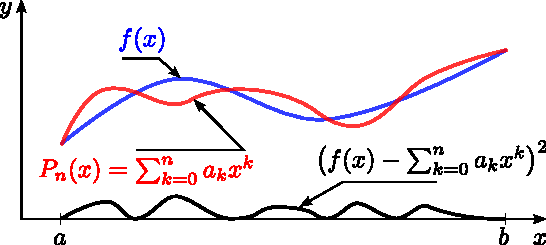
\includegraphics[width=1.0\textwidth]{figs/fig-01.pdf}
\end{center}
\pause

\[P_n(x) = a_n x^n + a_{n-1} x^{n-1} + \cdots + a_1 x + a_0 = \sum_{k=0}^n a_k x^k \]
\[ E \equiv E_2(a_0, a_1, \cdots, a_n) = \int_a^b \pow{f(x) - \sum_{k=0}^n a_k x^k}{2} \, dx \]  \pause

\cw{0.45}
\[ \frac{\partial E}{\partial a_j} = 0 \txt{para cada} j = 0, 1, \cdots, n \]

\begin{multline*}
    E = \int_a^b [f(x)]^2 dx -2 \sum_{k=0}^n a_k \int_a^b x^k f(x) \, dx \\
    + \int_a^b \pow{\sum_{k=0}^n a_k x^k}{2} \, dx
\end{multline*}

\[ \frac{\partial E}{\partial a_j} = -2 \int_a^b x^j f(x) \, dx +2 \sum_{k=0}^n a_k \int_a^b x^{j+k} \, dx \]
\alert{Ecuaciones normales} lineales ($n+1$):
\[ \sum_{k=0}^n a_k \int_a^b x^{j+k} \, dx = \int_a^b x^j f(x) \, dx \]
\flushright para cada $j = 0, 1, \cdots , n$.
\end{columns}
\end{frame}

\begin{frame}
    \textbf{Ejemplo:} aproximar $f(x) = \sen \pi x$ por un polinomio de grado 2 en $[0, 1]$.

\begin{columns}
\cw{0.6}
Ecuaciones normales:
\begin{align*}
    a_0 \int_0^1 1 \, dx + a_1 \int_0^1 x \, dx + a_2 \int_0^1 x^2 \, dx &= \int_0^1 \sen \pi x \, dx \\
    a_0 \int_0^1 x \, dx + a_1 \int_0^1 x^2 \, dx + a_2 \int_0^1 x^3 \, dx &= \int_0^1 x \, \sen \pi x \, dx \\
    a_0 \int_0^1 x^2 \, dx + a_1 \int_0^1 x^3 \, dx + a_2 \int_0^1 x^4 \, dx &= \int_0^1 x^2 \, \sen \pi x \, dx \\
\end{align*}

\begin{mathcols}
a_0 + \frac{1}{2} a_1 + \frac{1}{3} a_2 &= \frac{2}{\pi} \\
\frac{1}{2} a_0 + \frac{1}{3} a_1 + \frac{1}{4} a_2 &= \frac{1}{\pi} \\
\frac{1}{3}a_0 + \frac{1}{4} a_1 + \frac{1}{5} a_2 &= \frac{\pi^2 - 4}{\pi^3} \\
\changecol
&\txt{Solución} & \\
    a_0 &= \frac{12 \pi^2 - 120}{\pi^3} \approx -0.050465 \\
    a_1 &= -a2 = \frac{720 - 60 \pi^2}{\pi^3} \approx 4.12251
\end{mathcols}

\cw{0.4}
\begin{center}
    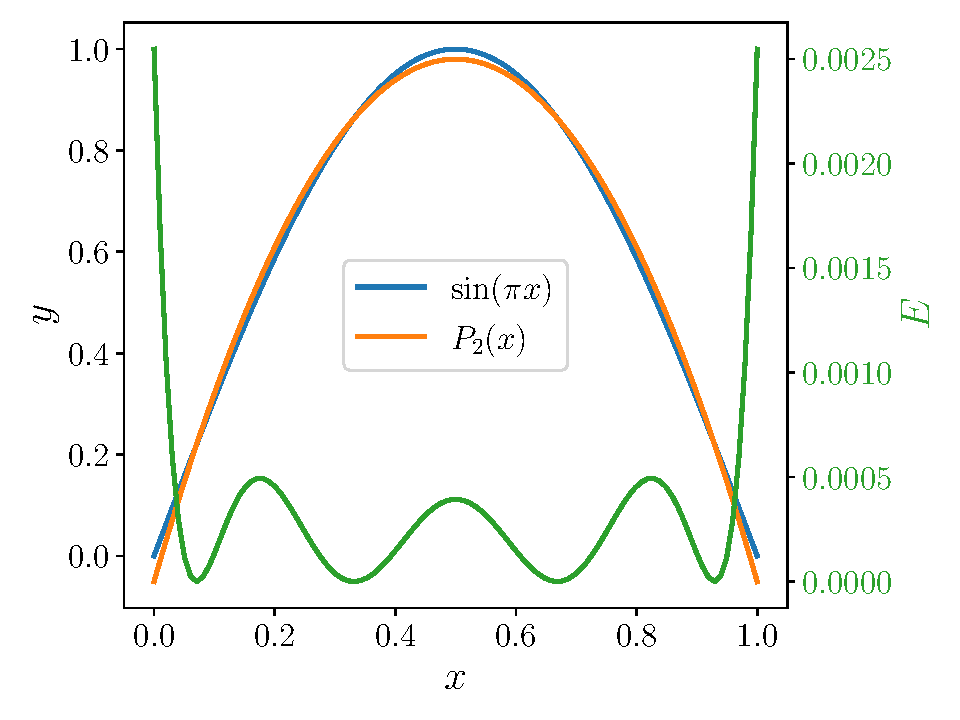
\includegraphics[width=1.0\textwidth]{figs/fig-02.pdf}
\end{center}

\end{columns}
\end{frame}

\begin{frame}
    \begin{columns}[t]
\cw{0.4}
\textbf{Problemas:}
\begin{itemize}
\item matriz de Hilbert
\begin{align*}
    H_{ij} &= \int_a^b x^{j+k} \, dx = \frac{b^{j+k+1} - a^{j+k+1}}{j + k + 1} \\
    \bm{H} &= \begin{bmatrix}
        1 & \frac{1}{2} & \frac{1}{3} \\
        \frac{1}{2}& \frac{1}{3} & \frac{1}{4} \\
        \frac{1}{3}& \frac{1}{4} & \frac{1}{5} \\
    \end{bmatrix} \\
        \cond(\bm{H}) &\approx 524.05678
\end{align*} \pause
\item No es fácil obtener $P_{n+1}(x)$ si ya tenemos $P_n(x)$
\end{itemize} \pause

\cw{0.55}
\begin{definition}[ Funciones linealmente independientes ]
Se dice que el conjunto de funciones $\{ \phi_0, \cdots, \phi_n \}$ es \textbf{linealmente independiente} (LI) en $[a, b]$ si
\[ P(x) = c_0 \phi_0(x) + c_1 \phi_1(x) + \cdots + c_n \phi_n(x) = 0, \forall x \in [a, b] \]
entonces $c_0 = c_1 = \cdots = c_n = 0$. De lo contrario, se dice que el conjunto de funciones es \textbf{linealmente dependiente}.
\end{definition}  \pause

\begin{theorem}[Polinomios LI]
    Si para cada $j = 0, 1, \cdots, n$, $\phi_j(x)$ es un polinomio de grado $j$, entonces el conjunto $\{ \phi_0, \cdots, \phi_n \}$ es LI en cualquier intervalo $[a, b]$.
\end{theorem}

\end{columns}
\end{frame}

\begin{frame}
    \textbf{Ejemplo.} Si $\phi_0(x) = 2, \phi_1(x) = x-3, \phi_2(x) = x^2 + 2x+7$ y $Q(x) = a_0 + a_1 x + a_2 x^2$, mostrar que existen constantes $c_0, c_1, c_2$ tales que $Q(x) = c_0 \phi_0(x) + c_1 \phi_1(x) + c_2 \phi_2(x)$.
\vspace{1em} \pause

\begin{columns}[t]
\cx
Por el teorema anterior, $\{\phi_0, \phi_1, \phi_2 \}$ es LI en cualquier $[a, b]$. Además:
\begin{align*}
1 &= \frac{1}{2}\phi_0(x) \\
x &= \phi_1(x) + 3 = \phi_1(x) + \frac{3}{2} \phi_0(x) \\
    x^2 &= \phi_2(x) - 2 x - 7 \\ 
        &= \phi_2(x) - 2 \left[ \phi_1(x) + \frac{3}{2} \phi_0(x) \right] - 7 \left[ \frac{1}{2} \phi_0(x) \right] \\
        &= \phi_2(x) -2 \phi_1(x) - \frac{13}{2} \phi_0(x)
\end{align*} \pause

\cx
Entonces:
\begin{align*}
    Q(x) &= a_0 \left[ \frac{1}{2} \phi_0 \right] + a_1 \left[ \phi_1(x) + \frac{3}{2} \phi_0(x)  \right] \\
         &+ a_2 \left[ \phi_2(x) - 2\phi_1(x) - \frac{13}{2} \phi_0(x) \right] \\
         &= \left( \frac{1}{2} a_0 + \frac{3}{2} a_1 - \frac{13}{2} a_2 \right) \phi_0(x)\\
         &+ [a_1 - 2 a_2] \phi_1(x) + a_2 \phi_2(x)
\end{align*}
\end{columns} \pause

\begin{theorem}[]
    Si $\Pi_n$ denota el conjunto de todos los polinomios de grado a lo sumo $n$, y $\{\phi_0(x), \phi_1(x), \cdots, \phi_n(x) \}$ es un conjunto de polinomios LI en $\Pi_n$, entonces \textbf{cualquier} polinomio en $\Pi_n$ se puede escribir como combinación lineal de $\phi_0(x), \phi_1(x), \cdots, \phi_n(x)$.
\end{theorem}

\end{frame}

\begin{frame}
    \begin{columns}[t]
\cw{0.45}
\begin{definition}[Función de peso]
    Una función integrable $w$ se denomina \textbf{función de peso} en el intervalo $I$ si $w(x) \geq 0, \forall x \in I$, pero $w(x) \not\equiv 0$ en cualquier subintervalo de $I$
\end{definition} \pause

Ejemplo: 
\[ w(x) = \frac{1}{\sqrt{1 - x^2}} \]
\begin{center}
    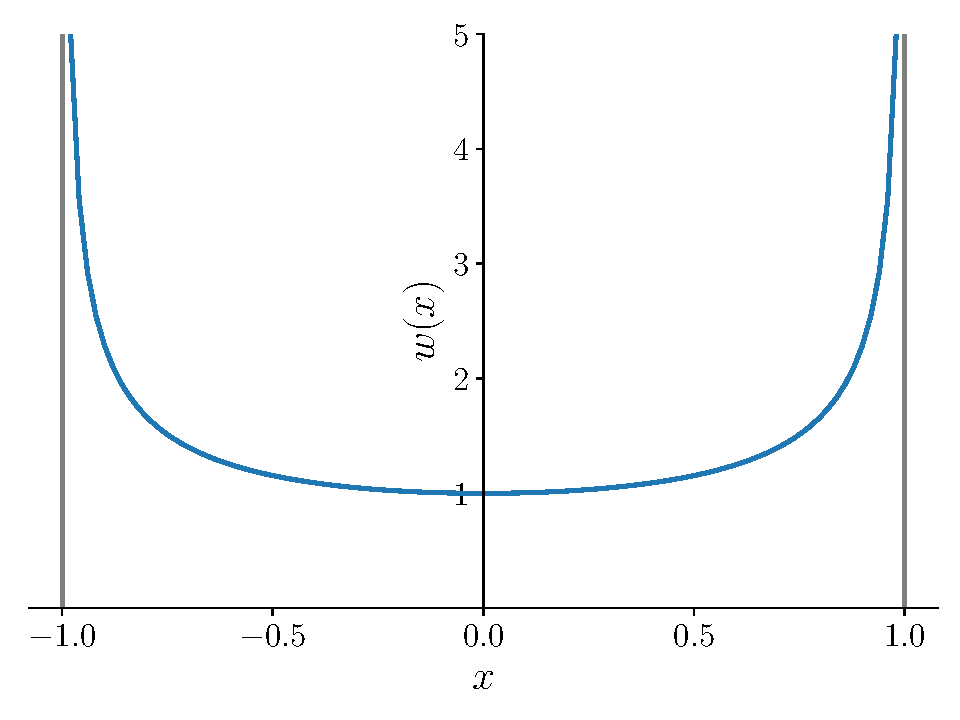
\includegraphics[width=0.9\textwidth]{figs/fig-03.pdf}
\end{center} \pause

\cw{0.55}
\begin{definition}[Funciones ortogonales]
    Se dice que $\{\phi_0, \phi_1, \cdots, \phi_n\}$ es un \textbf{conjunto ortogonal de funciones} en el intervalo $[a, b] $ respecto de la función de peso $w(x)$ si
    \[ \langle \phi_k, \phi_j \rangle_w = \int_a^b w(x) \phi_k(x) \phi_j(x) \, dx = 
        \begin{cases}
            0, & j \neq k, \\
            \alpha_j > 0, & j = k
        \end{cases}
    \]
Si además $\alpha_j = 1$ para cada $j = 0, 1, 2, \cdots, n$, se dice que el conjunto es \textbf{ortonormal}.
\end{definition} \pause

Ejemplo: $\{ \cos nx, \sen mx \}, n, m = 0, 1,  \cdots$ es ortogonal en $[-\pi, \pi]$ con $w(x) = 1$:
\begin{mathcols}
    \langle \cos nx, \cos mx \rangle_w &= 0 \\
    \langle \sen nx, \sen mx \rangle_w &= 0 \\
    \langle \cos nx, \sen mx \rangle_w &= 0 \\
    \changecol
    \langle \cos nx, \cos nx \rangle_w &= \pi \\
    \langle \sen nx, \sen nx \rangle_w &= \pi \\
    n \neq m
\end{mathcols}
\end{columns}
\end{frame}

\begin{frame}
\begin{columns}[t]
\cx
\begin{theorem}[]
    Si $\{\phi_0, \cdots, \phi_n \}$ es un conjunto ortogonal de funciones en un intervalo $[a, b]$ respecto de la función de peso $w(x)$, entonces la aproximación por mínimos cuadrados para $f$ en $[a, b]$ respecto de $w$ es:
    \[P(x) = \sum_{j=0}^n a_j \phi_j(x) \]
    donde para cada $j = 0, 1, \cdots, n$:
    \[ a_j = \frac{1}{\alpha_j} \langle f, \phi_j \rangle_w \]
\end{theorem} \pause

\cx
\begin{theorem}[]
    El conjunto de polinomios $\{\phi_0, \phi_1, \cdots, \phi_n\}$ definido de la siguiente forma es ortogonal en $[a, b]$ respecto de la función de peso $w(x)$:
    \[ \phi_0(x) \equiv 1, \; \phi_1(x) = x - B_1, \forall x \in [a, b] \]
    donde 
    \[ B_1 = \frac{ \langle x \phi_0, \phi_0 \rangle_w} {\langle \phi_0, \phi_0 \rangle_w} \]
    y cuando $k \geq 2$:
    \[ \phi_k(x) = (x - B_k) \phi_{k-1}(x) - C_k \phi_{k-2}(x), \, \forall x \in [a, b] \]
    donde
    \begin{mathcols}
        B_k &= \frac{ \langle x \phi_{k-1}, \phi_{k-1} \rangle_w } { \langle \phi_{k-1}, \phi_{k-1} \rangle_w } 
        \changecol
        C_k = \frac{ \langle x \phi_{k-1}, \phi_{k-2} \rangle_w }{\langle \phi_{k-2}, \phi_{k-2} \rangle_w }
    \end{mathcols} 
\end{theorem}
\centering {\small (Proceso de Gram-Schmidt)}
\end{columns}
\end{frame}

\begin{frame}
\begin{columns}[t]
\cx
\textbf{Polinomios de Legendre.}

$\{P_n(x) \}$ es ortogonal en $[-1, 1]$ con $w(x) \equiv 1$. Usando Gram-Schmidt con $P_0(x) \equiv 1$:
\[ B_1 = \frac{\int_{-1}^1 x \, dx}{\int_{-1}^1 dx} = 0, \, P_1(x) = (x - B_1) P_0(x) = x \] \pause
Luego:
\[ B_2 = \frac{\int_{-1}^1 x^3 \, dx}{\int_{-1}^1 x^2 \,dx} = 0, \, C_2(x) = \frac{\int_{-1}^1 x^2 \, dx}{\int_{-1}^1 1 \,dx} = \frac{1}{3} \]
\begin{align*}
    P_2(x) &= (x - B_2) P_1(x) - C_2 P_0(x) \\
           &= (x - 0) x - \frac{1}{3} 1 \\
           &= x^2 - \frac{1}{3}
\end{align*} \pause

\cx
\begin{align*}
    P_3(x) &= x P_2(x) - \frac{4}{15} P_1(x) = x^3 - \frac{3}{5} x \\
    P_4(x) &= x^4 - \frac{6}{7} x^2 + \frac{3}{35}, \, P_5(x) = x^5 - \frac{10}{9} x^3 + \frac{5}{21} x
\end{align*} \pause

\begin{center}
    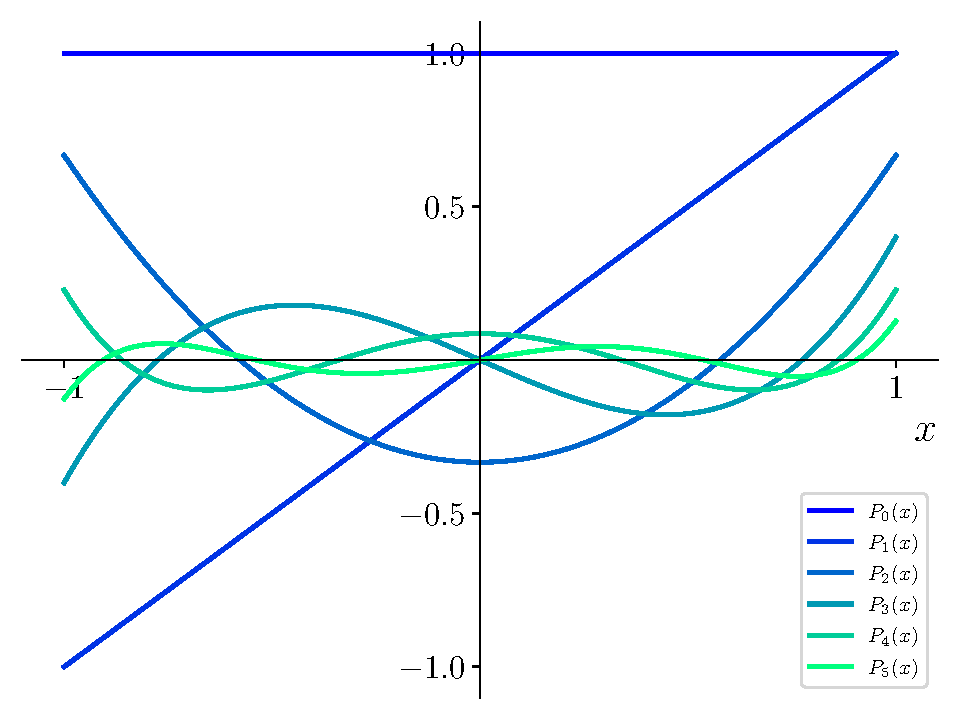
\includegraphics[width=0.9\textwidth]{figs/fig-04.pdf}
\end{center}
\end{columns}
\end{frame}

\begin{frame}[fragile]
\begin{columns}[t]
\cw{0.45}
\textbf{Ejemplo:} Python
\pycode[firstline=1, lastline=22]{figs/plot-05.py}

\cw{0.5}
\pycode[firstline=24]{figs/plot-05.py}
\end{columns}
\end{frame}

\begin{frame}
    \begin{center}
        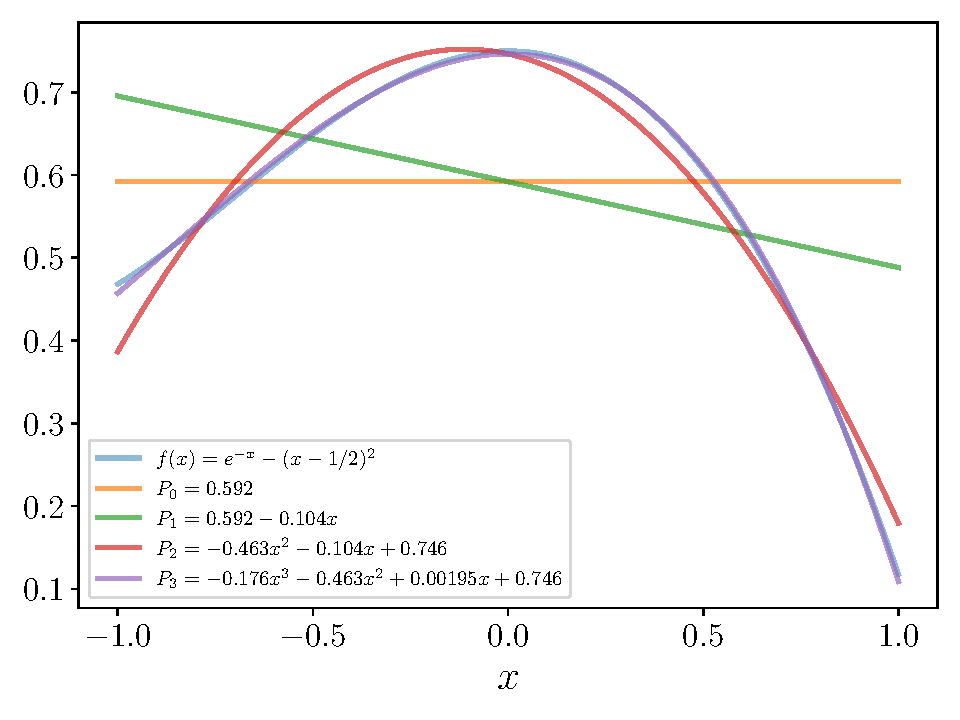
\includegraphics[width=0.8\textwidth]{figs/fig-05.pdf}
    \end{center}
\end{frame}

\begin{frame}
\begin{columns}[t]
\cx
\textbf{Polinomios de Chebyshev.}

$\{ T_n(x)\}$ es ortogonal en $(-1, 1)$ con función de peso $w(x) = (1-x^2)^{-1/2}$. Para $x \in [-1, 1]$:
\[ T_n(x) = \cos[n \arccos x], \; n \geq 0 \] \pause \vspace{-2em}
\[ T_0(x) = \cos 0 = 1 \txt{y} T_1(x) =\cos(\arccos x) = x \] \pause
Para $n \geq 1$, $\theta = \arccos x$:
\[ T_n(\theta(x)) \equiv T_n(\theta) = \cos (n \theta), \: \theta \in [0, \pi] \]
Relación de recurrencia:
\begin{align*}
T_{n+1}(\theta) &= \cos(n+1) \theta = \cos \theta \cos(n \theta) - \sen \theta \sen (n \theta) \\
T_{n-1}(\theta) &= \cos(n-1) \theta =  \cos \theta \cos(n \theta) + \sen \theta \sen (n \theta) 
\end{align*}
Sumando: 
\[ T_{n+1}(\theta) = 2 \cos \theta \cos(n \theta) - T_{n-1}(\theta) \] \pause

\cx
Regresando a $x = \cos \theta$, para $n \geq 1$:
\begin{align*}
    T_{n+1} &= 2 x \cos(n \arccos x) - T_{n-1}(x) \\
    T_{n+1}(x) &= 2 x T_n(x) - T_{n-1}(x)
\end{align*} \pause
Dado que $T_0(x) = 1$ y $T_1(x) = x$:
\begin{align*}
T_2(x) &= 2 x T_1(x) - T_0(x) = 2 x^2 -1 \\
T_3(x) &= 2 x T_2(x) - T_1(x) = 4 x^3 - 3 x \\
T_4(x) &= 2 x T_3(x) - T_2(x) = 8 x^4 - 8 x^2 + 1
\end{align*}

\begin{center}
    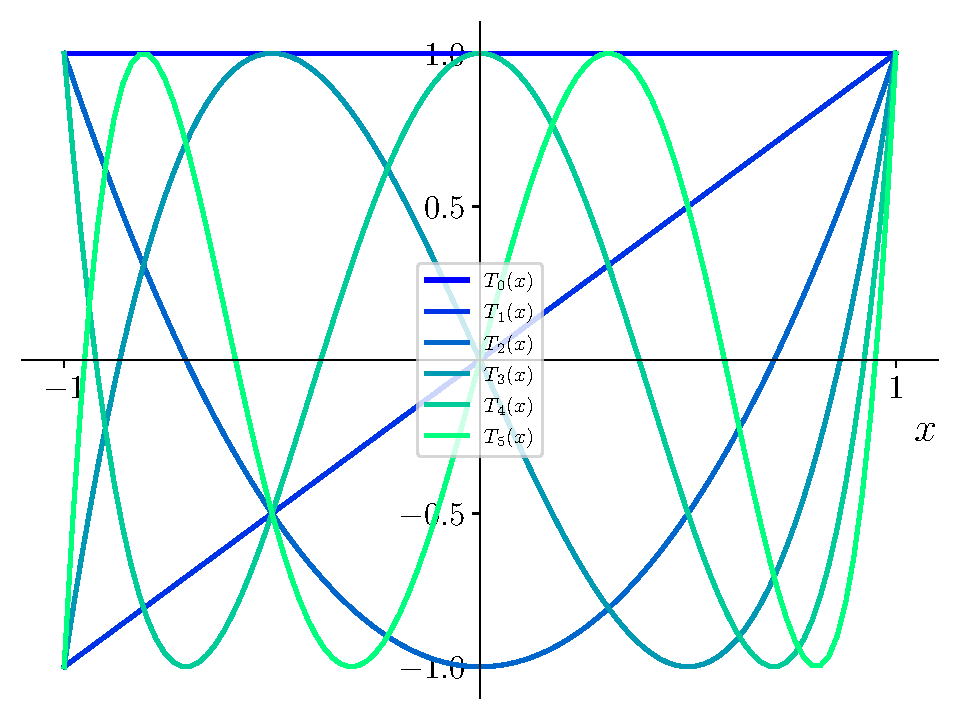
\includegraphics[width=0.8\textwidth]{figs/fig-06.pdf}
\end{center}
\end{columns}
\end{frame}

\begin{frame}
\begin{columns}[t]
\cx
\textbf{ Ortogonalidad de polinomios de Chebyshev }

\[ \int_{-1}^1 \frac{T_n(x) T_m(x)}{\sqrt{1 - x²}} \, dx = \int_{-1}^1 \frac{\cos(n \arccos x) \cos(m \arccos x)}{\sqrt{1 - x^2}} dx \]
Reintroducimos $\theta = \arccos x$:
\begin{align*}
d\theta &= -\frac{1}{\sqrt{1 - x^2}} dx \\
\int_{-1}^1 \frac{T_n(x) T_m(x)}{\sqrt {1 - x^2}} dx &= -\int_{\pi}^0 \cos(n \theta) \cos(m \theta) \, d\theta \\
  &= \int_{0}^{\pi} \cos(n \theta) \cos(m \theta) \, d\theta 
\end{align*}
Para $n \neq m$:
\[ \cos(n \theta) \cos(m \theta) = \frac{1}{2}[\cos(n+m) \theta + \cos(n-m)\theta] \]

\cw{0.25}
\vspace{7em}

Entonces:
\begin{align*}
    \langle T_n, T_m \rangle_w &= \frac{1}{2} \int_0^{\pi} \cos[(n+m) \theta] \, d\theta \\
      &+\frac{1}{2} \int_0^{\pi} \cos[(n-m) \theta] \, d\theta \\
      &= \left[ \frac{\sen[(n+m) \theta]}{2(n+m)} + \frac{\sen[(n-m) \theta]}{2(n-m)} \right]_0^{\pi}  \\
      &= 0
\end{align*}
y
\[ \langle T_n, T_n \rangle_w = 
    \begin{cases}
    \frac{\pi}{2}, &n \geq 1 \\
    \pi, &n = 0
\end{cases} \]
\end{columns}
\end{frame}

\begin{frame}
\begin{columns}[c]
\cx
\textbf{Reducción de grado de polinomio:}

\[ q(x) = x^5 - 4 x^4 + x^3 - x - 3 \]

Aproximación por:
\[ P_4(x) = c_0 + c_1 T_1(x) + c_2 T_2(x) + c_3 T_3(x) + c_4 T_4(x) \]
donde
\[ c_j = \frac{\langle q, T_j \rangle_w}{\langle T_j, T_j \rangle_w} \] \pause

\textbf{Resultado:} ver \texttt{code/plot-07.py}.
\[ P(x) = - 4.0 x^4 + 2.25 x^3 - 1.31 x - 3.0 \]

\cx
\begin{center}
    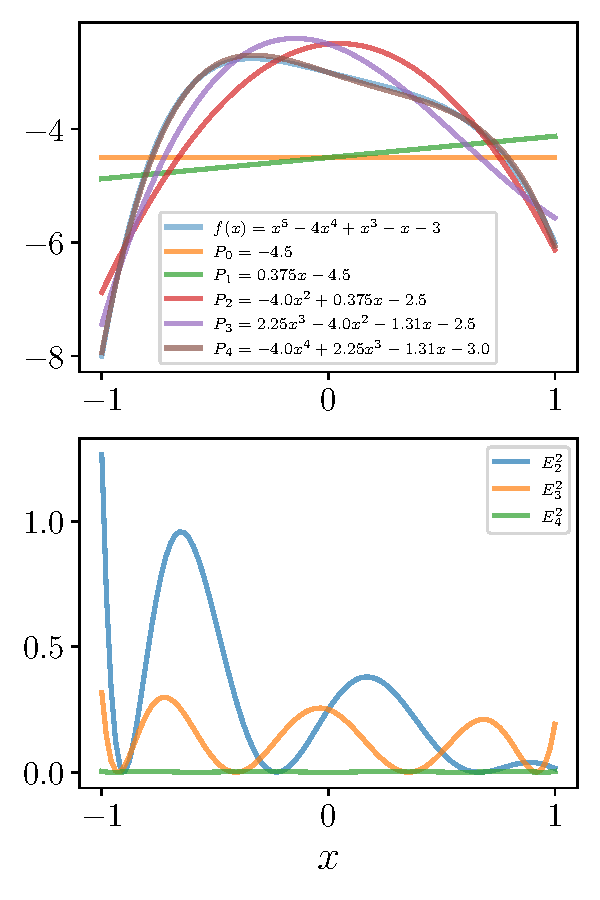
\includegraphics[height=1.0\textheight]{figs/fig-07.pdf}
\end{center}


\end{columns}
\end{frame}


%% =======================

\section*{Bibliografía}
\begin{frame}[allowframebreaks]{Lecturas recomendadas}
\begin{itemize}
    \item \fullcite{burden2017}. Capítulo 8.
    \item \fullcite{salgado2023}. Capítulo 11.
    \item \fullcite{quarteroni2000}. Capítulo 10.
    \item \fullcite{kreyszig2011}. Capítulo 25.9.
\end{itemize}
\end{frame}


\end{document}

